%%%%%%%%%%%%%%%%%%%%%%%%%%%%%%%%%%%%%%%%%%%%%%%%%%%%%%%%%%%%%%%
%
% Welcome to Overleaf --- just edit your LaTeX on the left,
% and we'll compile it for you on the right. If you open the
% 'Share' menu, you can invite other users to edit at the same
% time. See www.overleaf.com/learn for more info. Enjoy!
%
% Note: you can export the pdf to see the result at full
% resolution.
%
%%%%%%%%%%%%%%%%%%%%%%%%%%%%%%%%%%%%%%%%%%%%%%%%%%%%%%%%%%%%%%%
% Author: Till Tantau
% Source: The PGF/TikZ manual

\documentclass{standalone}

\usepackage{pgf}
\usepackage{tikz}
\usetikzlibrary{arrows,automata}
\usepackage[latin1]{inputenc}


\begin{document}
% [->,>=stealth',shorten >=1pt,auto,node distance=2cm,  semithick]
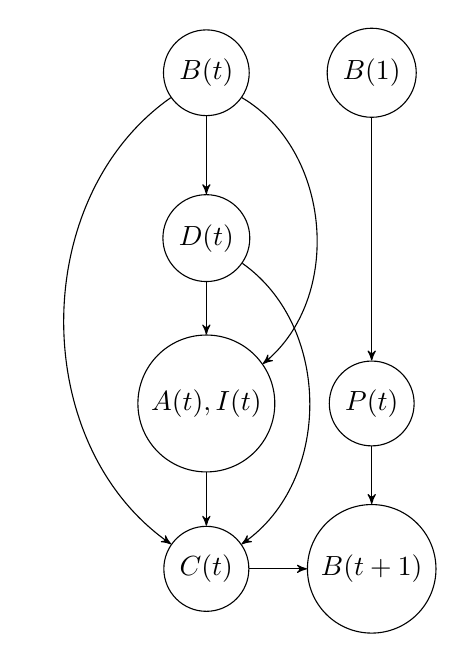
\begin{tikzpicture}
[->,>=stealth',node distance=2.1cm,>=stealth',bend angle=55,auto] 
  \tikzstyle{every state}=[fill=white,draw=black,text=black]

  \node[state] (B)                    {$ B(t)$};
  \node[state]         (D) [below of=B] {$D(t)$};
  \node[state]         (A) [below of=D] {$A(t),I(t)$};
  \node[state]         (C) [below of=A] {$C(t)$};
  \node[state]         (B1) [right of=B]       {$ B(1)$};
  \node[state]         (P) [right of=A]       {$P(t)$};
  \node[state]         (B1p) [right of=C]       {$B(t+1)$};
  \path (B) edge              node {} (D)
            edge [bend left]  node {} (A)
            edge [bend right]  node {} (C)
        (A) edge              node {} (C)
        (D) edge              node {} (A)
            edge [bend left]  node {} (C)
        (B1) edge             node {} (P)
        (P) edge             node {} (B1p)
        (C) edge             node {} (B1p)
            ;
        % (D) edge              node {} (A)
        % (E) edge [bend left]  node {} (A);
\end{tikzpicture}
% edge [loop below] node {1,1,R} (D)
%  edge [loop above] node {1,1,L} (B)
           
\end{document}